\section{Hardware}
\label{section:hardware}

The hardware used in this work constitutes a mobile 3D scanner called "lemonbot". This scanner's core components are a 2D laser scanner and a camera mounted on top of a pan and tilt unit. The other components are a mini computer, a battery and a wireless router. All the components are assembled on a tripod, according to the [esquemático do tripé]: the ptu is connected to the top of the tripod shaft, and the laser and camera is connected to the ptu moving link; the battery, computer wireless router and ptu driver is placed on a support in the legs of the ptu; a cable harness runs through the tripod's shaft connecting all parts to the host computer.
The host computer can be remotely controlled, via a remote connection (ssh), by connecting the client device (usually a computer) through the wireless network created by the router. This is specially useful to make the repetitive task of acquisitions faster and more agile.

\subsection{2D Laser Scanner}

One of the objectives of this work is to try different 2D laser scanners, to try to find the one that fits best for this kind of application. We chose four 2D laser scanners, trying to get a representative sample of all the market. This laser scanners differ in different aspects, as for example price, size, weight and working range. In \cref{table:laserscanners}, a comparison of the characteristics of this laser scanners are specified. 

\begin{figure}
    \centering
    \subfloat[Sick~LMS100]{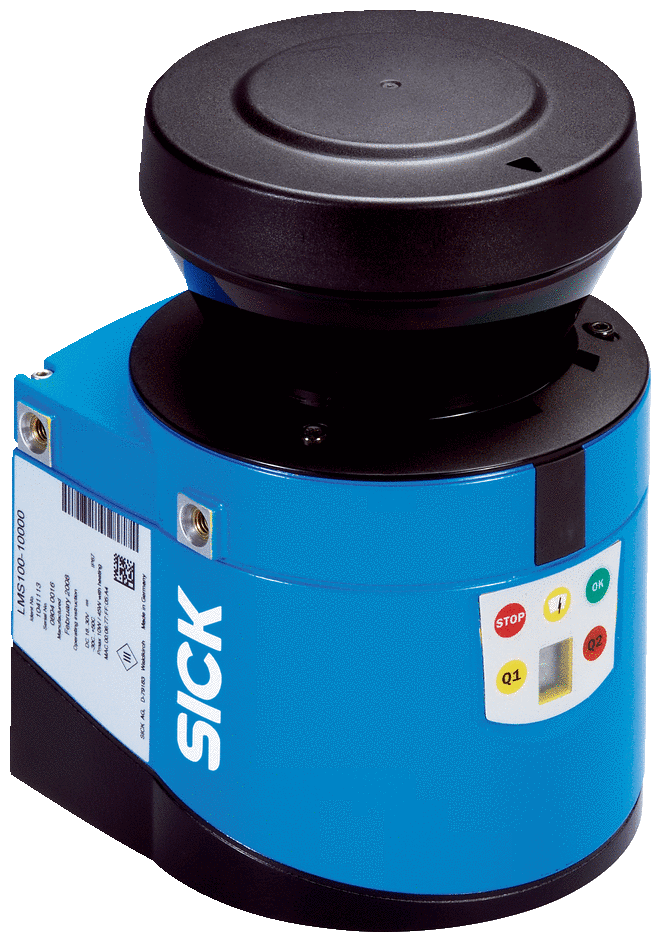
\includegraphics[width=3cm]{03-lms100}}%
    \qquad\qquad
    \subfloat[Sick~LMS200]{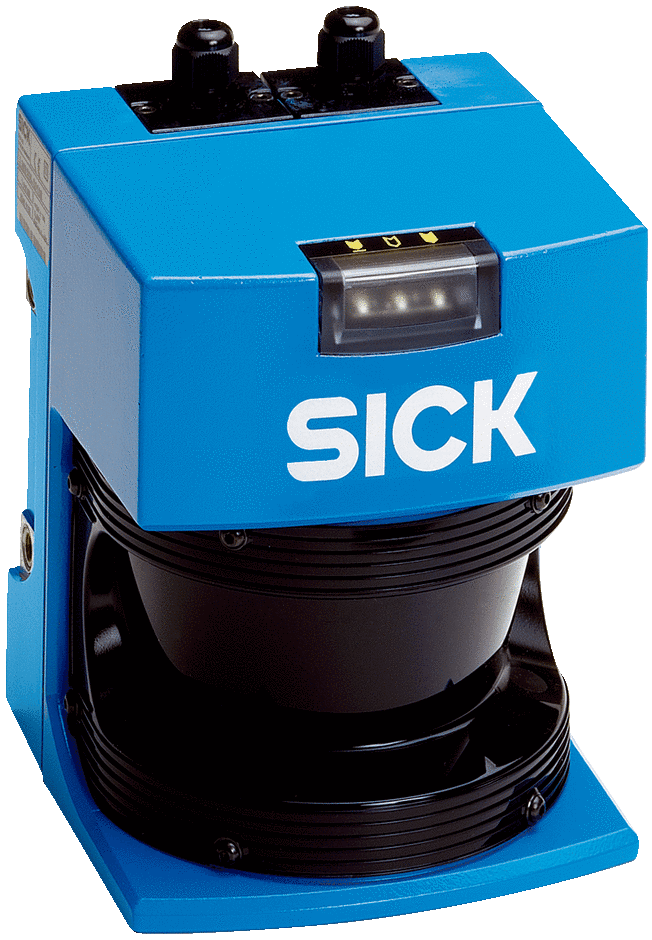
\includegraphics[width=3cm]{03-lms200}}%

    \subfloat[Hokuyo~URG04LX]{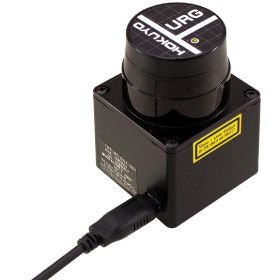
\includegraphics[width=4cm]{03-hokuyo_urg_04}}%
    \qquad\qquad
    \subfloat[Hokuyo~UTM-30LX]{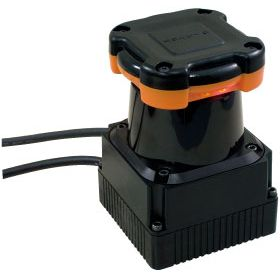
\includegraphics[width=4cm]{03-hokuyo_utm_30lx}}%

    \caption{2D Laser scanners used}
    \label{figure:laserscanners}
\end{figure}

\begin{sidewaystable}
    \caption{2D laser scanners used and their characteristics}
    
    \centering    
    \begin{longtabu}{@{} >{\bfseries}X[] X[] X[] X[] X[] @{}}
        \toprule
                            & Sick~LMS100       & Sick~LMS200    & Hokuyo's~URG04LX  & Hokuyo~UTM-30LX    \\
        \toprule
        Application         & \multicolumn{4}{c}{Indoor}                                                        \\
        Safety Class        & \multicolumn{4}{c}{Class 1 (eye-safe)}                                            \\
        Light source        & Infrared (\SI{905}{\nano\meter})
                            & Infrared (\SI{905}{\nano\meter})
                            & Red (\SI{785}{\nano\meter})
                            & Infrared (\SI{905}{\nano\meter})      \\
        Aperture angle      & \SI{270}{\degree}
                            & \SI{180}{\degree}
                            & \SI{240}{\degree}
                            & \SI{270}{\degree}    \\
        Scanning Frequency  & \SI{10}{\hertz}
                            & \SI{50}{\hertz}
                            & \SI{10}{\hertz}
                            & \SI{40}{\hertz}      \\
        Angular Resolution  & \SI{0.25}{\degree}
                            & \SI{0.25}{\degree}
                            & \SI{0.36}{\degree}
                            & \SI{0.25}{\degree}   \\
        Working Range       & \SIrange{0.5}{20}{\meter} 
                            & \SIrange{0}{80}{\meter}
                            & \SIrange{0.02}{5.6}{\meter}
                            & \SIrange{0.1}{30}{\meter} \\
        Systematic Error    & \SI{\pm20}{\milli\meter} 
                            & \SI{\pm15}{\milli\meter}
                            & NA
                            & NA \\
        Statistical Error   & \SI{\pm 12}{\milli\meter}
                            & \SI{\pm 5}{\milli\meter} 
                            & \SI{\pm 3}{\percent} 
                            & \SIrange{0.1}{10}{\meter}: \SI{\pm 30}{\milli\meter};
                              \SIrange{10}{30}{\meter}: \SI{\pm 50}{\milli\meter} \\
        Size                &
                            &
                            &
                            & \\
        Price               & 5000\euro
                            &
                            &
                            &  \\
        \bottomrule
    \end{longtabu}


    \label{table:laserscanners_characteristics}
\end{sidewaystable}

\subsection{Camera}

The camera used in this work was a PointGrey Flea3 FL3-GE-28S4 Camera (\cref{figure:pointgrey_flea3}), which is extensively used in industrial and traffic applications. The high quality of the images, the programming interface and it's compact size and weight makes it perfect for computer vision applications in industrial environment. The most relevant characteristics are represented on the \cref{table:pointgrey_flea3_characteristics}.

\begin{figure}[h]
    \centering
    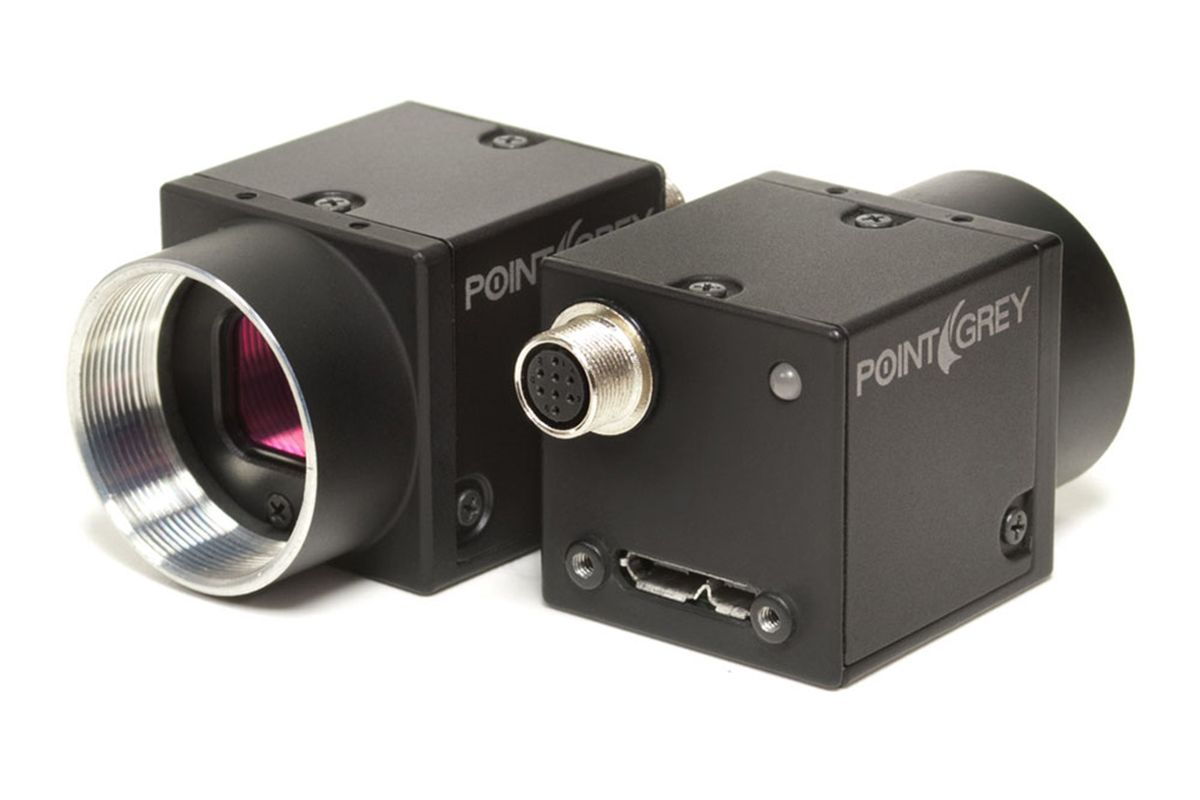
\includegraphics[width=0.5\textwidth]{03-pointgrey_flea3}
    \caption{PointGrey Flea3 FL3-GE-28S4}
    \label{figure:pointgrey_flea3}
\end{figure}

\begin{table}

    \caption{Characteristics of the PointGrey Flea3 FL3-GE-28S4 Camera}

    \centering
    \begin{tabu} spread 0.2\textwidth {>{\bfseries}X[l] X[r]}
        \toprule

        Resolution  & $1920 \times 1448$    \\
        Framerate   & 15 fps                \\
        Pixels      & \SI{2.8}{\mega P}     \\
        Color       & Yes                   \\
        Interface   & GigE Vision           \\
        Power       & \SIrange{12}{24}{\volt} \\
        Dimensions  & \SI{29 x 29 x 30}{\milli\meter} \\
        \bottomrule
    \end{tabu}

    \label{table:pointgrey_flea3_characteristics}

\end{table}

\subsection{Pan Tilt Unit}

Both the laser and camera are placed on top of a pan and tilt unit for their movement. The ptu chosen was the FLIR PTU-D46 (\cref{figure:pan_tilt_d46}), which is a compact and light module with the following characteristics:

\begin{itemize}
    \item Small form factor,
    \item Maximum payload weight of \SI{4}{\kilo\gram},
    \item \SI{+-159}{\degree} pan range and \SIrange{-47}{+31}{\degree} tilt range.
    \item \SI{60}{\degree \per \second} maximum speed.
    \item Angular resolution of \SI{0.0032}{\degree},
    \item Communication to the host via serial interface.
\end{itemize}

\begin{figure}[h]
    \centering
    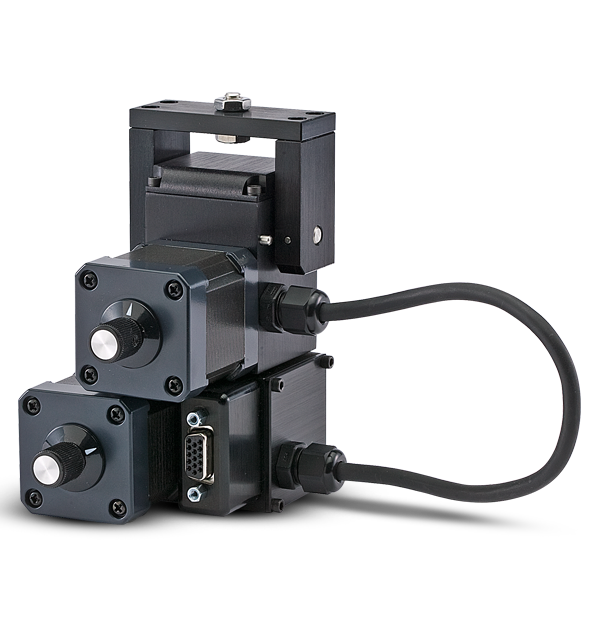
\includegraphics[width=0.5\textwidth]{03-ptu_d46}
    \caption{FLIR PTU-D46}
    \label{figure:pan_tilt_d46}
\end{figure}